\section{Escopo do Projeto}
A proposta de projeto é uma aplicação \textit{web} voltada para auxiliar no acompanhamento da evolução no rendimento dos alunos nas atividades escolares. 

\subsection{Modelagem}
Para detalhar melhor a aplicação, foi feita a análise de requisitos, a elaboração das histórias de usuários, a criação do backlog do produto, a modelagem de dados e elaboração dos protótipos.

\subsubsection{Análise de Requisitos}
A análise de requisitos é fundamental para o desenvolvimento da aplicação, pois a partir dela pode ser levantadas as funcionalidades e restrições que o sistema deve apresentar. Para isso, foram levantados os requisitos funcionais e não funcionais do sistema.

\subsubsubsection{Requisitos Funcionais}
Os requisitos funcionais levantados são descritos no \autoref{quadro-requisitosfuncionais}.
\begin{quadro}[htb]
\centering
\ABNTEXfontereduzida
\caption{\label{quadro-requisitosfuncionais}Requisitos funcionais}
\begin{tabular}{|m{2.2cm}|m{9.6cm}|m{2.2cm}|}
\hline
{\thead{Identificador}} & \thead{Descrição} & \thead{Categoria}   \\ \hline
    RF01 &  O sistema deve permitir o cadastro de um administrador por outro administrador &  Essencial \\ \hline
    RF02 & O sistema deve permitir o cadastro de escola pelo administrador  & Essencial \\\hline
    RF03 & O sistema deve permitir o envio de e-mail para completar o cadastro de escola & Essencial  \\ \hline
    RF04 & O sistema deve permitir a visualização de um resumo do uso do sistema para o administrador & Importante  \\ \hline
    RF05 & O sistema deve permitir uma definição de senha no primeiro acesso &  Essencial   \\ \hline
    RF06 &  O sistema deve permitir a realização do login & Essencial \\ \hline  
    RF07 &  O sistema deve permitir a recuperação de senha &  Essencial \\ \hline 
    RF08 &  O sistema deve permitir a revogação de acesso de um administrador e de um gestor &  Essencial  \\ \hline   
    RF09 &  O sistema deve permitir a desativação de uma escola &  Essencial \\ \hline
    RF10 &  O sistema deve permitir o cadastro de turmas pelo gestor & Essencial  \\ \hline    
    RF11 &  O sistema deve permitir o cadastro de professores pelo gestor & Essencial  \\ \hline    
    RF12 &  O sistema deve permitir a atribuição de um ou mais professores e seus respectivos alunos às turmas &  Essencial \\ \hline  
    RF13 & O sistema deve permitir ao professor somente a exibição das turmas atribuídas ao mesmo  & Essencial \\ \hline 
    RF14 &  O sistema deve permitir o cadastro de atividades pelo professor & Essencial  \\ \hline  
    RF15 &  O sistema deve permitir o detalhamento das atividades & Essencial  \\ \hline  
    RF16 & O sistema deve permitir ao professor somente a exibição das atividades das turmas atribuídas ao mesmo  & Essencial \\ \hline  
    RF17 &  O sistema deve permitir a entrega e visualização das atividades &  Essencial \\ \hline  
    RF18 &  O sistema deve permitir a visualização e atribuição de correções & Essencial  \\ \hline  
    RF19 &  O sistema deve permitir o cadastro de conquistas pelo professor &  Essencial \\ \hline  
    RF20 &  O sistema deve permitir a listagem de conquistas personalizada para cada perfil & Essencial  \\ \hline  
    RF21 &  O sistema deve permitir a visualização do ranking personalizada para cada perfil &  Essencial \\ \hline  
    RF22 &  O sistema deve permitir o cálculo e visualização de pontuações &  Essencial \\ \hline  
    RF23 &  O sistema deve permitir o detalhamento das conquistas & Essencial  \\ \hline  
    RF24 &  O sistema deve permitir a visualização de dashboards para acompanhar o desempenho & Importante  \\ \hline  
    RF25 &  O sistema deve permitir a utilização dos conceitos de gamificação presentes nessa aplicação, em outras aplicações &  Importante \\ \hline  

\end{tabular}
\fonte{Os autores}
\end{quadro}
\FloatBarrier

\subsubsubsection{Requisitos Não Funcionais}
Os requisitos não funcionais levantados são descritos no \autoref{quadro-requisitosnaofuncionais}.
\begin{quadro}[htb]
\centering
\ABNTEXfontereduzida
\caption{\label{quadro-requisitosnaofuncionais}Requisitos não funcionais}
\begin{tabular}{|m{2.2cm}|m{9.6cm}|m{2.2cm}|}
\hline
{\thead{Identificador}} & \thead{Descrição} & \thead{Categoria}   \\ \hline
    RNF01 & O sistema deve possuir telas responsivas para que o usuário possa ter a mesma experiência independente do dispositivo  &  Usabilidade \\ \hline
    RNF02 & O sistema deve seguir o protocolo HTTPS & Segurança \\\hline
    RNF03 & O sistema deve respeitar a LGPD & Segurança  \\ \hline
    RNF04 & O sistema deve permitir a sua escalabilidade no futuro por meio do código e da hospedagem escolhida & Desempenho  \\ \hline
\end{tabular}
\fonte{Os autores}
\end{quadro}
\FloatBarrier


\subsubsection{Histórias de Usuário}
Com os requisitos levantados, foi-se possível elaborar as histórias de usuário para estabelecer as funcionalidades do sistema. 

\begin{itemize}
    \item\textbf{Funcionalidade}: Cadastro de administrador
    
    Eu, como administrador, quero criar outro administrador, para que alguém possa me ajudar nas tarefas administrativas do sistema.
    \begin{itemize}
        \item Cenário: Cadastro bem sucedido  
        \par Dado que estou na tela de cadastro de usuários na visão do administrador
        \par Quando eu preencher todos os dados corretamente
        \par E apertar o botão de Criar
        \par Então receberei uma mensagem de usuário criado com sucesso
    \end{itemize}   
    \begin{itemize}
        \item Cenário: Cadastro mal sucedido  
        \par Dado que estou na tela de cadastro de usuários na visão do administrador
        \par Quando eu preencher algum dado incorretamente
        \par Então não conseguirei clicar no botão de Criar, pois o botão estará inativo
    \end{itemize}       
    \begin{itemize}
        \item Cenário: E-mail já cadastrado  
        \par Dado que estou na tela de cadastro de usuários na visão do administrador
        \par Quando eu preencher algum dado de um administrador que já está cadastrado no sistema
        \par Então receberei uma mensagem que o e-mail já está cadastrado no sistema
    \end{itemize}    

\item\textbf{Funcionalidade}: Cadastro de escola
    
    Eu, como administrador, gostaria de cadastrar escolas para meus clientes.
    \begin{itemize}
        \item Cenário: Cadastro bem sucedido  
        \par Dado que estou na tela de cadastro de escolas na visão do administrador
        \par Quando eu preencher todos os dados corretamente
        \par E apertar o botão de Criar
        \par Então receberei uma mensagem de escola criada com sucesso
    \end{itemize}   
    \begin{itemize}
        \item Cenário: Cadastro mal sucedido  
        \par Dado que estou na tela de cadastro de escolas na visão do administrador
        \par Quando eu preencher algum dado incorretamente
        \par Então não conseguirei clicar no botão de Criar, pois o botão estará inativo
    \end{itemize}    

\item\textbf{Funcionalidade}: \glspl{dashboard} do uso do sistema
    
    Eu, como administrador, quero visualizar a quantidade de professores, de alunos e de gestores cadastrados, para que eu possa tomar decisões com base nesses dados de quem está usando o sistema.
    \begin{itemize}
        \item Cenário: Visualização do uso do sistema 
        \par Dado que estou na tela de login
        \par Quando eu fazer o login com o perfil de administrador
        \par Então conseguirei ver as principais quantidades dos usuários que usam o sistema
    \end{itemize} 

\item\textbf{Funcionalidade}: Primeiro acesso
    
    Eu, como usuário do sistema, gostaria de poder definir a minha senha durante o primeiro acesso a aplicação para garantir a segurança do acesso.
    \begin{itemize}
        \item Cenário: Definição de senha  
        \par Dado que o meu usuário já está cadastrado
        \par E recebi o \gls{link} de acesso à aplicação por e-mail
        \par Quando eu clicar nesse \gls{link}
        \par E ser redirecionado à tela de primeiro acesso
        \par Então conseguirei definir a minha senha
    \end{itemize}

\item\textbf{Funcionalidade}: Login
    
    Eu, como usuário do sistema, gostaria de fazer o login na aplicação para garantir a privacidade dos meus dados.
    \begin{itemize}
        \item Cenário: Login bem sucedido  
        \par Dado que estou na tela de login
        \par Quando eu preencher o e-mail e a senha corretamente
        \par E apertar o botão de Login
        \par Então irei para a tela inicial da aplicação
    \end{itemize}   
    \begin{itemize}
        \item Cenário: Login mal sucedido  
        \par Dado que estou na tela de login
        \par Quando eu preencher algum dado incorretamente
        \par Então receberei uma mensagem de erro
    \end{itemize}    

\item\textbf{Funcionalidade}: Recuperação de senha
    
    Eu, como usuário do sistema, gostaria de poder recuperar minha senha.
    \begin{itemize}
        \item Cenário: Cadastro de nova senha
        \par Dado que estou na tela de login
        \par Quando eu clicar no botão de esqueci a senha
        \par E digitar o e-mail válido
        \par E clicar em redefinir senha
        \par Então receberei um e-mail com um novo \gls{link} 
        \par E por esse \gls{link} serei redirecionado para uma tela de redefinição de senha
        \par E conseguirei cadastrar uma nova senha
    \end{itemize}    
    \begin{itemize}
        \item Cenário: Inserção de e-mail inválido
        \par Dado que estou na tela de login
        \par Quando eu clicar no botão de esqueci a senha
        \par E digitar o e-mail que não seja válido
        \par Então não conseguirei clicar no botão de redefinir senha
    \end{itemize}    

\item\textbf{Funcionalidade}: Revogação de acessos de um administrador
    
    Eu, como administrador, quero revogar os acessos de outro administrador, para caso ele seja demitido da empresa.
    \begin{itemize}
        \item Cenário: Alteração do usuário
        \par Dado que estou na tela de usuários na visão do administrador
        \par E selecionei o usuário que desejo desativar
        \par Quando eu desselecionar o botão de ativo 
        \par E apertar o botão de Salvar
        \par Então receberei uma mensagem de usuário alterado com sucesso
    \end{itemize}   

\item\textbf{Funcionalidade}: Revogação de acessos de um gestor
    
    Eu, como administrador, quero revogar os acessos de um gestor e sua escola, para caso eles criem conteúdos inadequados.
    \begin{itemize}
        \item Cenário: Alteração do gestor
        \par Dado que estou na tela de gestores na visão do administrador
        \par E selecionei o gestor que desejo desativar
        \par Quando eu desselecionar o botão de ativo
        \par E apertar o botão de Salvar
        \par Então receberei uma mensagem de gestor alterado com sucesso
    \end{itemize}  

\item\textbf{Funcionalidade}: Desativação de uma escola
    
    Eu, como administrador, quero desativar a escola, para suspender o uso de seus usuários quando os mesmos estiverem em débito com a empresa.
    \begin{itemize}
        \item Cenário: Alteração da escola  
        \par Dado que estou na tela de cadastro de escolas na visão do administrador
        \par E selecionei a escola que desejo desativar
        \par Quando eu desselecionar o botão de ativo
        \par E apertar o botão de Salvar
        \par Então receberei uma mensagem de escola alterada com sucesso
    \end{itemize}   
    
\item\textbf{Funcionalidade}: Cadastro de turma
    
    Eu, como gestor, gostaria de cadastrar uma nova turma para os alunos do próximo ano letivo.
    \begin{itemize}
        \item Cenário: Cadastro bem sucedido  
        \par Dado que estou na tela de cadastro de turmas na visão do gestor
        \par Quando eu preencher todos os dados corretamente
        \par E apertar o botão de Criar
        \par Então receberei uma mensagem de turma criada com sucesso
    \end{itemize}   
    \begin{itemize}
        \item Cenário: Cadastro mal sucedido  
        \par Dado que estou na tela de cadastro de turmas na visão do gestor
        \par Quando eu preencher algum dado incorretamente
        \par Então não conseguirei clicar no botão de Criar, pois ele estará inativo
    \end{itemize}   

\item\textbf{Funcionalidade}: Cadastro de professor
    
    Eu, como gestor, gostaria de dar o cargo de professor a um novo usuário caso um novo professor seja contratado.
    \begin{itemize}
        \item Cenário: Cadastro bem sucedido  
        \par Dado que estou na tela de cadastro de professores na visão do gestor
        \par Quando eu preencher todos os dados corretamente
        \par E apertar o botão de Criar
        \par Então receberei uma mensagem de professor criado com sucesso
    \end{itemize}   
    \begin{itemize}
        \item Cenário: Cadastro mal sucedido  
        \par Dado que estou na tela de cadastro de professores na visão do gestor
        \par Quando eu preencher algum dado incorretamente
        \par Então não conseguirei clicar no botão de Criar, pois ele não estará ativo
    \end{itemize}   
    \begin{itemize}
        \item Cenário: E-mail já existente 
        \par Dado que estou na tela de cadastro de professores na visão do gestor
        \par Quando eu preencher os dados com um e-mail que já existe no sistema
        \par Então não conseguirei clicar no botão de Criar, pois ele não estará ativo
    \end{itemize}  

\item\textbf{Funcionalidade}: Cadastro de aluno
    
    Eu, como gestor, gostaria de cadastrar os alunos da minha escola para que eles possam acessar o sistema.
    \begin{itemize}
        \item Cenário: Cadastro bem sucedido  
        \par Dado que estou na tela de cadastro de alunos na visão do gestor
        \par Quando eu preencher todos os dados corretamente
        \par E apertar o botão de Criar
        \par Então receberei uma mensagem de aluno criado com sucesso
    \end{itemize}   
    \begin{itemize}
        \item Cenário: Cadastro mal sucedido  
        \par Dado que estou na tela de cadastro de alunos na visão do gestor
        \par Quando eu preencher algum dado incorretamente
        \par Então não conseguirei clicar no botão de Criar, pois ele não estará ativo
    \end{itemize}   
    \begin{itemize}
        \item Cenário: E-mail já existente 
        \par Dado que estou na tela de cadastro de alunos na visão do gestor
        \par Quando eu preencher os dados com um e-mail que já existe no sistema
        \par Então não conseguirei clicar no botão de Criar, pois ele estará inativo
    \end{itemize} 
    \begin{itemize}
        \item Cenário: Matrícula já existente 
        \par Dado que estou na tela de cadastro de alunos na visão do gestor
        \par Quando eu preencher os dados com uma matrícula que já existe no sistema
        \par Então não conseguirei clicar no botão de Criar, pois ele não estará ativo
    \end{itemize} 

\item\textbf{Funcionalidade}: Atribuição de professores e alunos
    
    Eu, como gestor, gostaria de atribuir professores e alunos as suas devidas turmas para facilitar a interação entre ambos os lados.
    \begin{itemize}
        \item Cenário: Cadastro de alunos e professores às turmas
        \par Dado que estou na tela turmas na visão do gestor
        \par Quando eu clicar em criar turmas
        \par E colocar os respectivos alunos e professores
        \par Então conseguirei atribuir alunos e professores às turmas
    \end{itemize}

\item\textbf{Funcionalidade}: Atribuição de dois professores 
    
    Eu, como gestor, gostaria de atribuir dois professores em uma mesma turma de alunos que pode ser dividida.
    \begin{itemize}
        \item Cenário: Cadastro de dois professores à mesma turma
        \par Dado que estou na tela turmas na visão do gestor
        \par Quando eu clicar em criar turmas
        \par E colocar os dois professores
        \par Então conseguirei dois professores à mesma turma
    \end{itemize}

\item\textbf{Funcionalidade}: Listagem de todas as turmas
    
    Eu, como gestor, gostaria de visualizar todas as turmas cadastradas para uma melhor administração das mesmas.
    \begin{itemize}
        \item Cenário: Visualização de todas as turmas 
        \par Dado que estou cadastrado como gestor no sistema
        \par Quando eu fazer o login
        \par E selecionar a opção turmas
        \par Então todas as turmas cadastradas na minha escola aparecerão em formato de lista
    \end{itemize}  

\item\textbf{Funcionalidade}: Listagem de turmas
    
    Eu como professor, gostaria de visualizar as turmas atribuídas a mim para postar meus conteúdos por turma.
    \begin{itemize}
        \item Cenário: Visualização de turmas 
        \par Dado que estou cadastrado como professor no sistema
        \par Quando eu fazer o login
        \par Então todas as turmas atribuídas para mim aparecerão em formato de abas
    \end{itemize}  

\item\textbf{Funcionalidade}: Cadastro de atividades
    
    Eu, como professor, gostaria de cadastrar atividades no sistema para que meus alunos façam.
    \begin{itemize}
        \item Cenário: Cadastro bem sucedido  
        \par Dado que estou na tela de cadastro de atividades na visão do professor
        \par Quando eu preencher todos os dados corretamente
        \par E apertar o botão de Criar
        \par Então receberei uma mensagem de atividade criada com sucesso
    \end{itemize}   
    \begin{itemize}
        \item Cenário: Cadastro mal sucedido  
        \par Dado que estou na tela de cadastro de atividades na visão do professor
        \par Quando eu preencher algum dado incorretamente
        \par Então não conseguirei clicar no botão de Criar
    \end{itemize}   

\item\textbf{Funcionalidade}: Definição das atividades
    
    Eu, como professor, gostaria de marcar se uma atividade é avaliativa ou não e se é entregável ou não para poder atribuir melhor as conquistas.
    \begin{itemize}
        \item Cenário: Alteração de atividades  
        \par Dado que estou na tela de atividades na visão do professor
        \par Quando eu clicar em criar atividade 
        \par Então conseguirei definir se a atividade é avaliativa e/ou entregável
    \end{itemize}

\item\textbf{Funcionalidade}: Listagem de atividades
    
    Eu, como aluno, gostaria de poder visualizar as minhas atividades ordenadas por data de vencimento, para não perder nenhum prazo de entrega.
    \begin{itemize}
        \item Cenário: Visualização de atividades 
        \par Dado que estou cadastrado como aluno no sistema
        \par Quando eu fazer o login
        \par Então todas as minhas atividades aparecerão em formato de lista por ordem de data de vencimento
    \end{itemize}   

\item\textbf{Funcionalidade}: Detalhamento de atividades
    
    Eu, como aluno, gostaria de visualizar todos os detalhes da atividade para não ter dúvidas sobre como realizá-la.
    \begin{itemize}
        \item Cenário: Visualização detalhada de atividades  
        \par Dado que estou na tela de atividades na visão do aluno
        \par Quando eu clicar na atividade desejada
        \par Então conseguirei ver os detalhes dessa atividade
    \end{itemize}  

\item\textbf{Funcionalidade}: Recebimento de atividades
    
    Eu, como professor, gostaria de receber as atividades no sistema para poder corrigi-las.
    \begin{itemize}
        \item Cenário: Visualização de atividades entregues
        \par Dado que estou na tela de atividades na visão do professor
        \par E seleciono a atividade que quero ver as entregas
        \par Quando eu clicar em visualizar entregas
        \par Então conseguirei ver as atividades e os alunos que enviaram
    \end{itemize}

\item\textbf{Funcionalidade}: Atribuição de \gls{feedback}
    
    Eu, como professor, gostaria de atribuir \gls{feedback} aos meus alunos das atividades para que possa retornar uma nota caso for avaliativa.
    \begin{itemize}
        \item Cenário: Inserção de \gls{feedback}
        \par Dado que estou na tela de atividades entregues na visão do professor
        \par E seleciono a atividade que desejo mandar o feedback
        \par Quando eu escrever o comentário do campo do feedback
        \par E clicar em Salvar
        \par Então estarei atribuindo um feedback para a atividade
    \end{itemize}

\item\textbf{Funcionalidade}: Visualização do \gls{feedback}
    
    Eu, como aluno, gostaria de ver o \gls{feedback} das correções das atividades que valem nota, para saber o que preciso melhorar.
    \begin{itemize}
        \item Cenário: Visualização de \gls{feedback}
        \par Dado que estou na tela de atividades na visão do aluno
        \par Quando eu clicar na atividade que desejo ver o feedback
        \par Então conseguirei ver o feedback do professor
    \end{itemize}

\item\textbf{Funcionalidade}: Cadastro de conquistas
    
    Eu, como gestor, gostaria de cadastrar diferentes tipos de conquistas para que os alunos possam alcançá-las.
    \begin{itemize}
        \item Cenário: Cadastro bem sucedido  
        \par Dado que estou na tela de cadastro de conquistas na visão do gestor
        \par Quando eu preencher todos os dados de todas as etapas corretamente
        \par E apertar o botão de Criar
        \par Então receberei uma mensagem de conquista criada com sucesso
    \end{itemize}   
    \begin{itemize}
        \item Cenário: Cadastro mal sucedido  
        \par Dado que estou na tela de cadastro de conquistas na visão do gestor
        \par Quando eu preencher algum dado incorretamente
        \par Então não conseguirei clicar no botão de Criar, pois ele estará inativo
    \end{itemize}   
    \begin{itemize}
        \item Cenário: Campo nulo
        \par Dado que estou na tela de cadastro de conquistas na visão do gestor
        \par Quando eu deixar de preencher algum dado no sistema
        \par Então não conseguirei clicar no botão de Criar, pois ele não estará ativo
    \end{itemize}   

\item\textbf{Funcionalidade}: Listagem de conquistas
    
    Eu, como aluno, gostaria de visualizar minhas conquistas pendentes, para que eu corra atrás de conquistá-las e subir no \gls{ranking}.
    \begin{itemize}
        \item Cenário: Visualização de conquistas 
        \par Dado que estou na tela inicial na visão do aluno
        \par Quando eu clicar para aparecer a barra lateral
        \par E clicar em ver conquistas
        \par Então todas as minhas conquistas pendentes aparecerão em cinza
    \end{itemize}  

\item\textbf{Funcionalidade}: Posição geral no \gls{ranking}
    
    Eu, como aluno mais inteligente da sala, gostaria de poder visualizar minha posição no \gls{ranking} geral da turma, para alimentar meu ego.
    \begin{itemize}
        \item Cenário: Visualização da posição no \gls{ranking}
        \par Dado que estou na tela inicial na visão do aluno
        \par Quando eu clicar para aparecer a barra lateral
        \par Então conseguirei ver a minha posição no \gls{ranking}
    \end{itemize}  

\item\textbf{Funcionalidade}: Omissão da posição do \gls{ranking}
    
    Eu, como aluno não tão bem empenhado, não gostaria que minha posição no \gls{ranking} seja visível para outros alunos, a não ser que eu esteja entre os primeiros da minha liga, para não sofrer \textit{bullying}.
    \begin{itemize}
        \item Cenário: Visualização do \gls{ranking} por turma
        \par Dado que estou na tela inicial na visão do aluno
        \par Quando eu clicar para aparecer a barra lateral
        \par Então não conseguirei ver a posição dos outros alunos que não seja a minha e os três primeiros
    \end{itemize}  

\item\textbf{Funcionalidade}: Pontuação
    
    Eu, como aluno, gostaria de ver minha pontuação geral, e a pontuação dos três primeiros do \gls{ranking} da minha liga, para saber o quanto eu preciso me esforçar para alcançá-los.
    \begin{itemize}
        \item Cenário: Visualização pontuação
        \par Dado que estou na tela inicial na visão do aluno
        \par Quando eu clicar para aparecer a barra lateral
        \par Então conseguirei ver a minha pontuação
    \end{itemize}  
 
\item\textbf{Funcionalidade}: Posição no \gls{ranking} por turma
    
    Eu, como professor, gostaria de ver o \gls{ranking} de cada turma para poder fazer o acompanhamento da mesma.
    \begin{itemize}
        \item Cenário: Visualização do \gls{ranking} por turma
        \par Dado que estou na tela inicial na visão do professor
        \par E com a barra lateral aberta
        \par Quando eu clicar em ver \gls{ranking} por turma
        \par Então serei redirecionado para a tela do \gls{ranking} por turma
    \end{itemize}  

\item\textbf{Funcionalidade}: Detalhamento de conquistas
    
    Eu como aluno, gostaria de saber quais as conquistas/pontuações mínimas eu preciso ter para avançar para próxima liga.
    \begin{itemize}
        \item Cenário: Visualização detalhada de conquistas  
        \par Dado que estou na tela de conquistas na visão do aluno
        \par Quando eu clicar na conquista desejada
        \par Então conseguirei ver os detalhes dessa conquista
    \end{itemize}  

\item\textbf{Funcionalidade}: \gls{ranking} de todas as turmas
    
    Eu, como gestor, gostaria de ver o \gls{ranking} de cada turma para poder fazer o acompanhamento das mesmas.
    \begin{itemize}
        \item Cenário: Visualização do \gls{ranking} de todas as turmas
        \par Dado que estou cadastrado como gestor no sistema
        \par Quando eu fazer o login
        \par E selecionar a opção \gls{ranking}
        \par Então todos os \glspl{ranking} das turmas cadastradas na minha escola aparecerão em formato de lista
    \end{itemize}

\item\textbf{Funcionalidade}: \glspl{dashboard} de desempenho
    
    Eu, como gestor, gostaria de ver o desempenho de cada turma e de alunos em particular para poder acompanhar cada caso com a devida atenção necessária.
    \begin{itemize}
        \item Cenário: Visualização dos dashboards 
        \par Dado que estou cadastrado como gestor no sistema
        \par Quando eu fazer o login
        \par Então todos os dashboards relacionados a minha escola aparacerão
    \end{itemize}   

\item\textbf{Funcionalidade}: Integração com o Moodle
    
    Eu, como gestor de uma escola, gostaria que o sistema pudesse se integrar ao Moodle para que eu adicione o conceito de gamificação para meus alunos sem que precise substituir o LMS utilizado na minha escola.
    \begin{itemize}
        \item Cenário: Integração 
        \par Dado que estou na tela inicial do Moodle
        \par Quando eu fazer o login 
        \par E ativar o plugin do Turma de Elite
        \par Então conseguirei ver os conceitos de gamificação do Turma de Elite no Moodle
    \end{itemize}  
\end{itemize} 

\subsubsection{Product Backlog}
Com as histórias de usuário definidas, foi montado o \gls{product-backlog} para definir a ordem de importância delas. A \autoref{product-backlog} representa o resultado da priorização, segundo cada funcionalidade.  
\begin{PAGINA-A3}

\begin{figure}[p]
    \centering 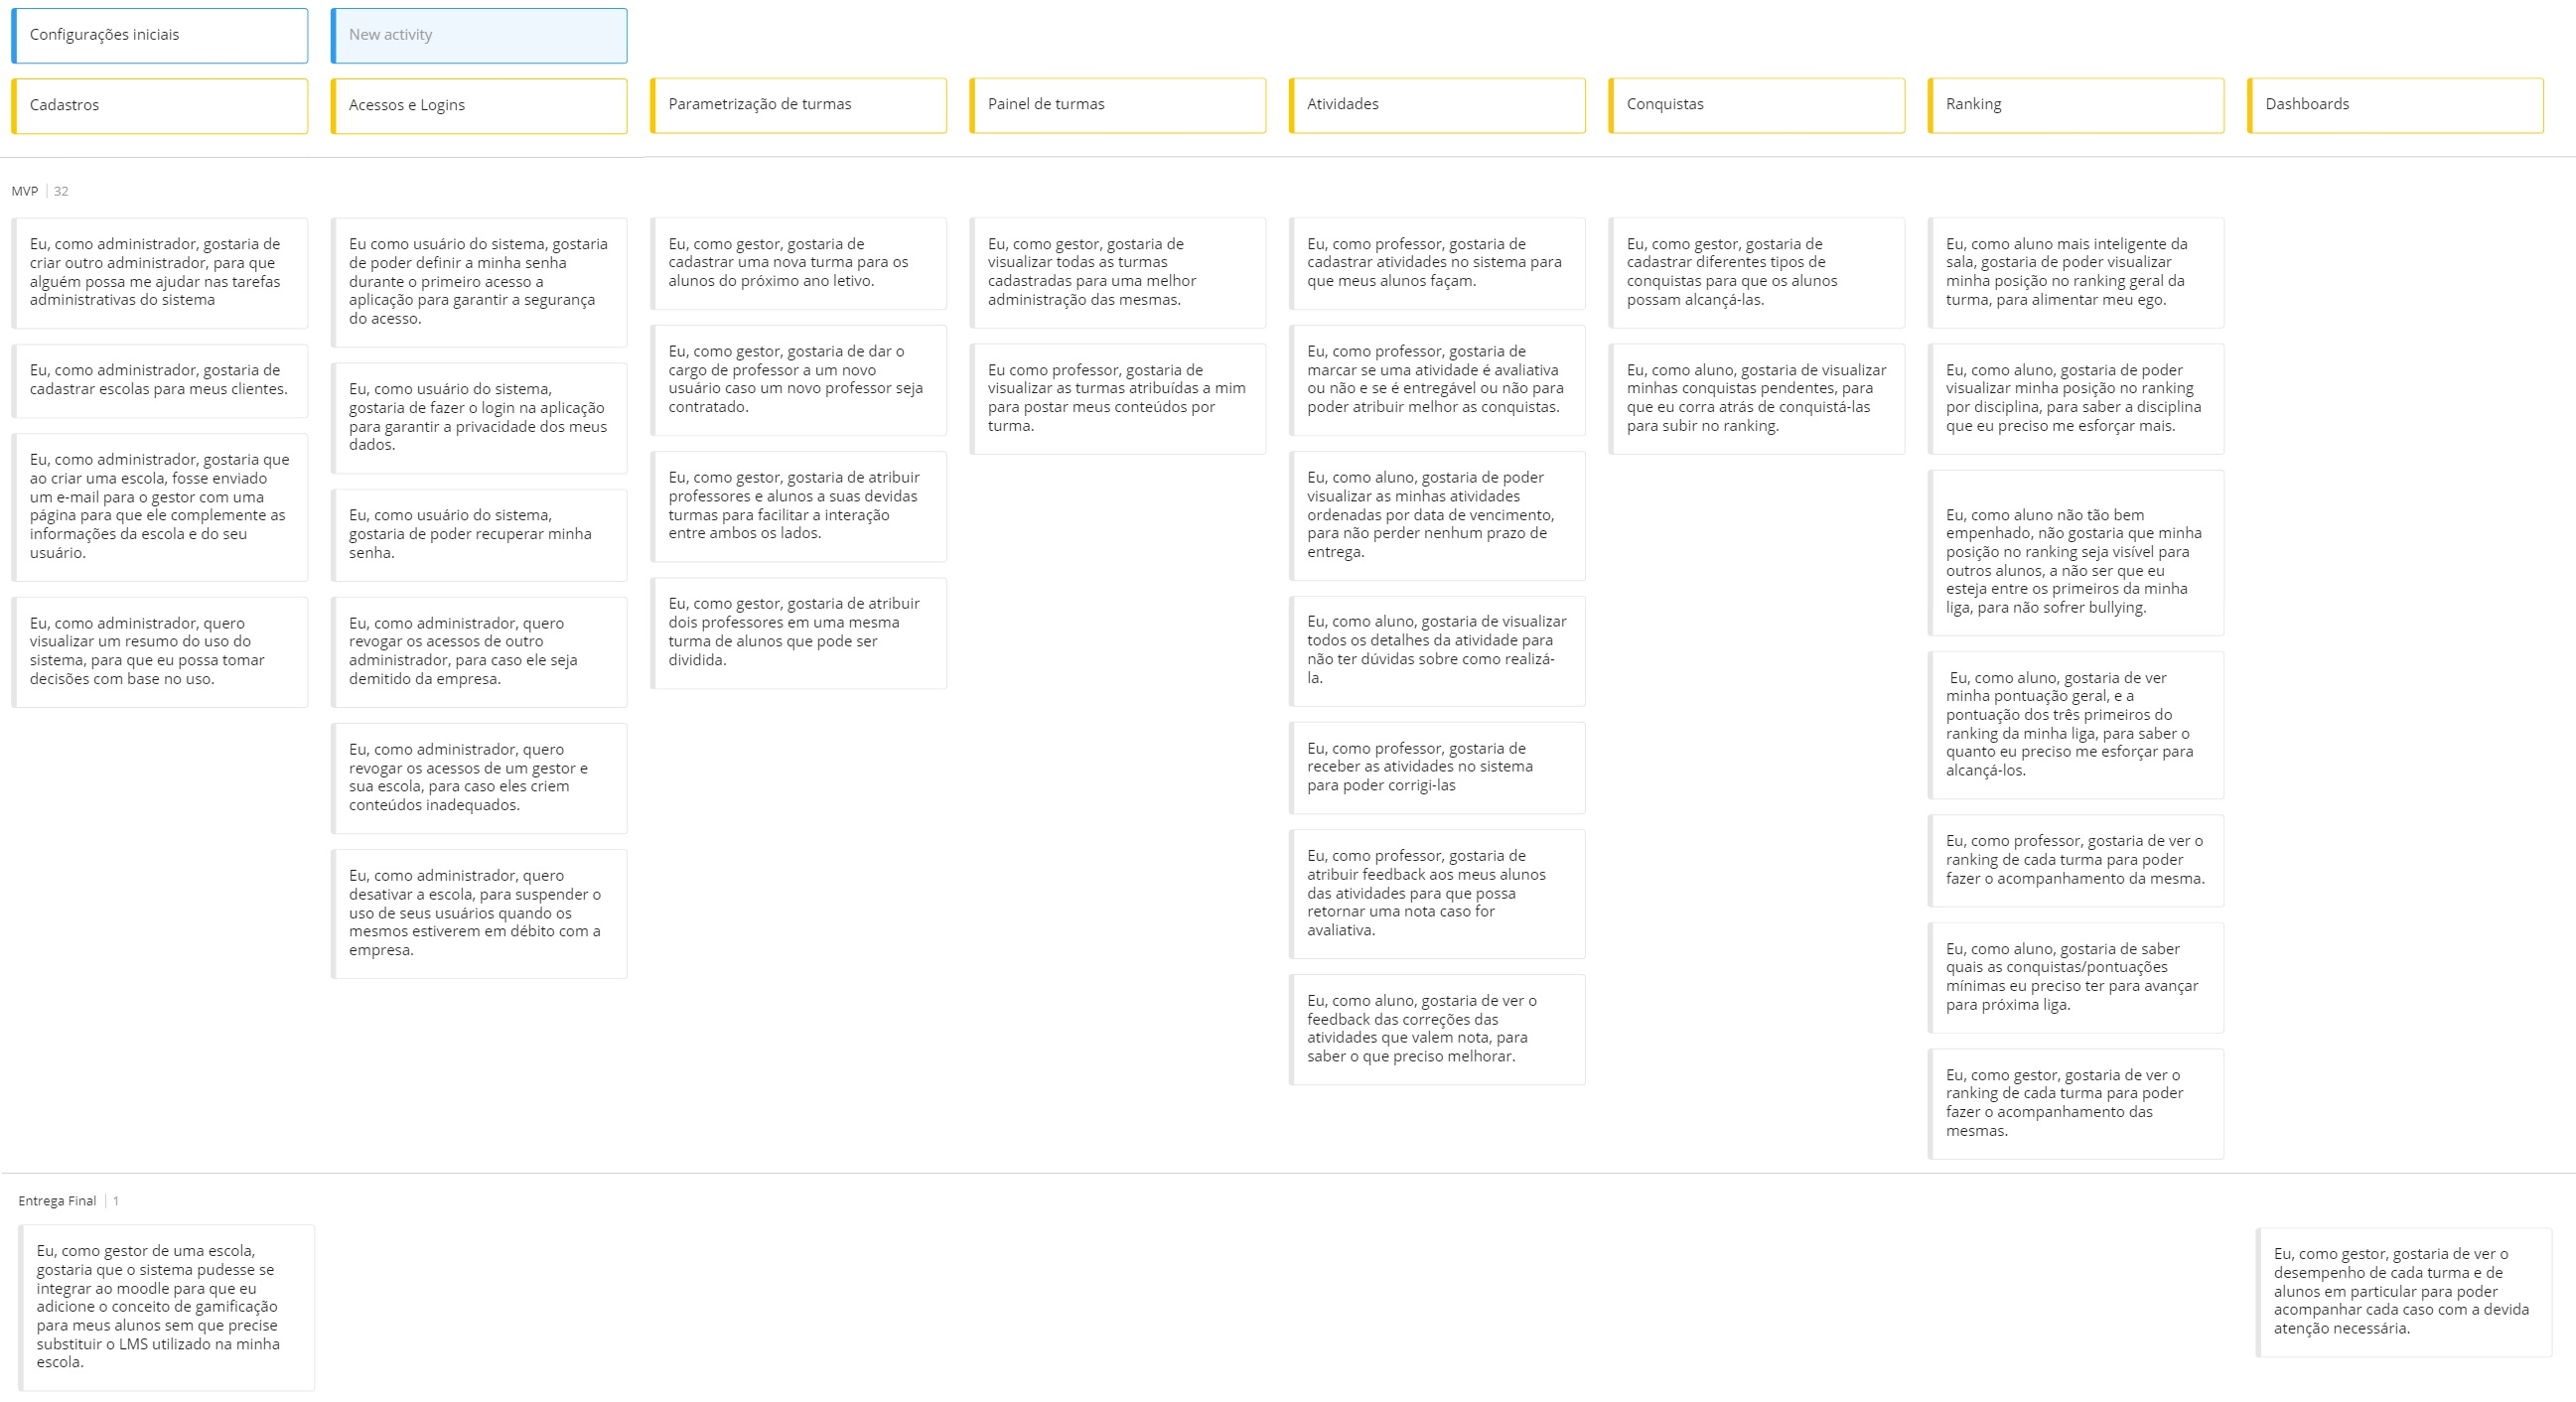
\includegraphics[height=\textheight,width=\textwidth,keepaspectratio]{imagens/UserStoryMappingFrameworkHD.jpg}
	\caption{\label{product-backlog}Product Backlog}
   \fonte{Os autores}
\end{figure}

\end{PAGINA-A3}

\subsubsection{MER e DER}
Para a modelagem de dados do projeto, foi elaborado o \ac{mer} da aplicação, segundo a \autoref{mer-figura}. E, para representá-lo, foi feito o \ac{der}, conforme demostra a \autoref{der-figura}.

\begin{PAGINA-A3}

\begin{figure}[p]
    \centering 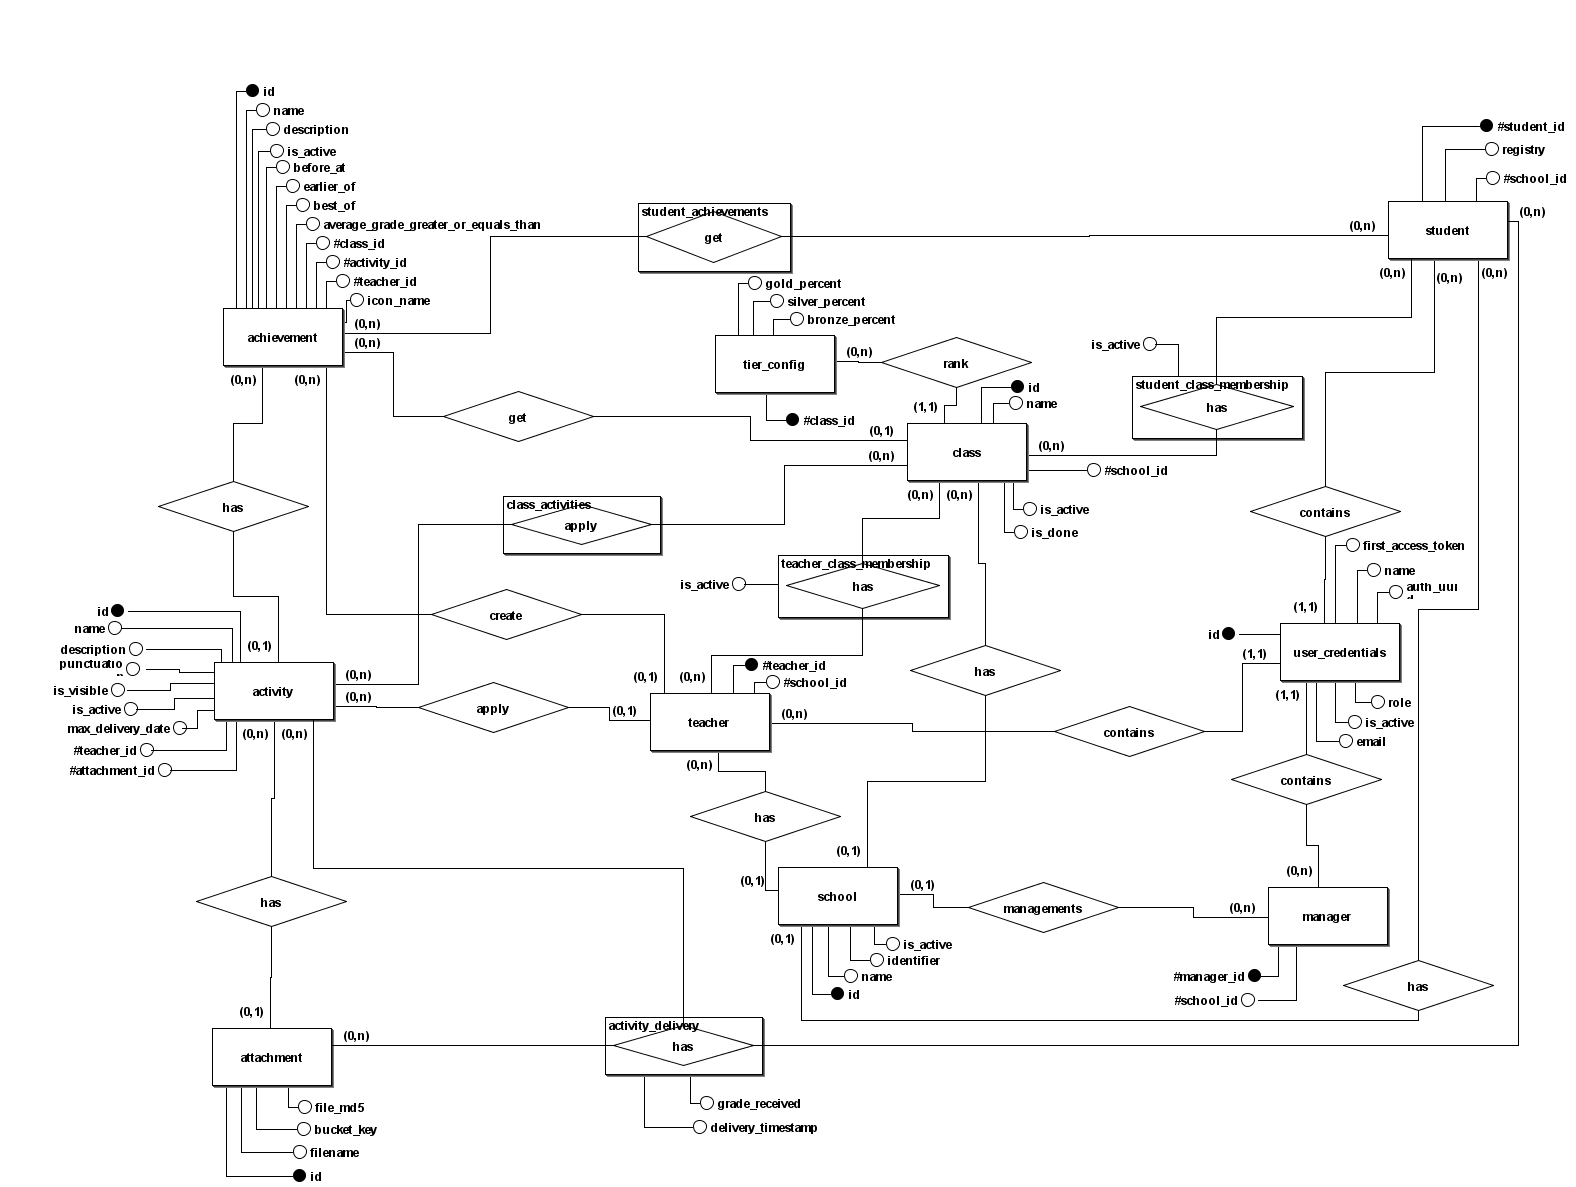
\includegraphics[height=\textheight,width=\textwidth,keepaspectratio]{imagens/ModeloConceitual.png}
	\caption{\label{mer-figura}Modelo Entidade Relacionamento}
   \fonte{Os autores}
\end{figure}

\end{PAGINA-A3}


\begin{PAGINA-A3}

\begin{figure}[p]
    \centering 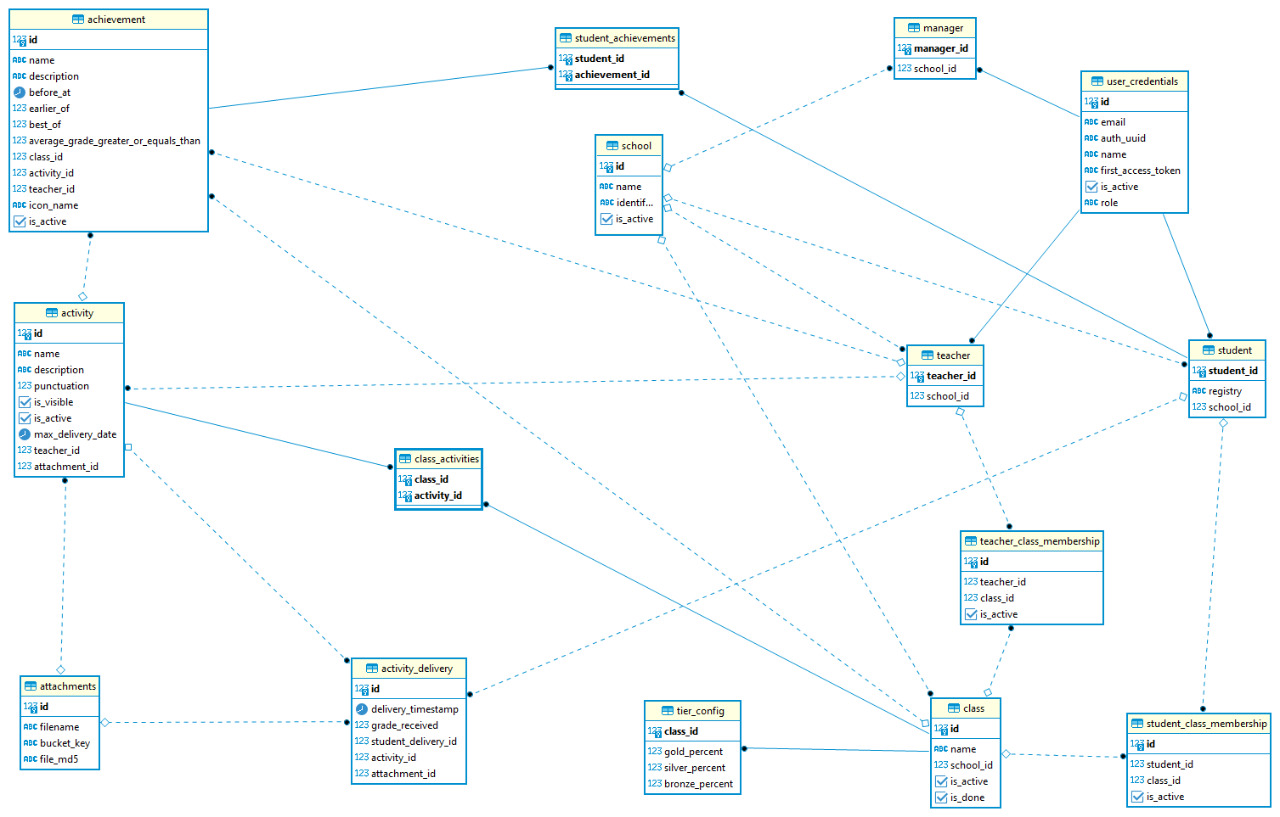
\includegraphics[height=\textheight,width=\textwidth,keepaspectratio]{imagens/der.jpg}
	\caption{\label{der-figura}Diagrama Entidade Relacionamento}
   \fonte{Os autores}
\end{figure}

\end{PAGINA-A3}

\subsubsection{Dicionário de Dados}

Neste momento, a aplicação possui 15 tabelas para armazenamento dos dados. O \autoref{quadro-tabelas-bd} apresenta todas as tabelas do sistema.

\begin{quadro}[htb]
\centering
\ABNTEXfontereduzida
\caption[Entidades do banco de dados]{Tabelas do banco de dados}
\label{quadro-tabelas-bd}
\begin{tabular}{|p{4.5cm}|}
  \hline
   \thead{Tabelas} \\
    \hline
    achievement \\
    \hline
    activity \\
    \hline
    activity\_delivery \\
    \hline
    attachments \\
    \hline
    class \\
    \hline
    class\_activities \\
    \hline
    manager \\
    \hline
    school \\
    \hline
    student \\
    \hline
    student\_achievements \\
    \hline
    student\_class\_membership \\
    \hline
    teacher \\
    \hline
    teacher\_class\_membership \\
    \hline
    tier\_config \\
    \hline
    user\_credentials \\
    \hline
\end{tabular}
\legend{Fonte: Os autores}
\end{quadro}
\FloatBarrier

A tabela \textit{achievement} contém todos os dados referentes às conquistas que poderão ser obtidas pelos alunos conforme a conclusão de tarefas. O \autoref{quadro-tabelabd-achievement} apresenta todos os atributos dessa tabela com suas respectivas características.

\begin{quadro}[htb]
\centering
\ABNTEXfontereduzida
\caption[Dicionário de Dados: Tabela achievement]{Dicionário de Dados: Tabela achievement}
\label{quadro-tabelabd-achievement}
\begin{tabular}{|l|m{3.0cm}|m{2.5cm}|m{1.0cm}|m{2.0cm}|m{2.0cm}|m{2.0cm}|}
  \hline
   \thead{Variável} & \thead{Descrição} & \thead{Tipo}  & \thead{Identi- \\ fica- \\ dor}  & \thead{Restrições \\ de \\ domínio} & Definições adicionais & \thead{Referências} \\
    \hline
      id & Atributo identificador da conquista & BIGINT & X & UNIQUE, NOT NULL & \makecell{AUTO\_\\INCREMENT} &  \\
      \hline
      name & Nome da conquista & VARCHAR(50) & & NOT NULL & &\\
      \hline
      description & Descrição da conquista & VARCHAR(240) & & NOT NULL &  & \\
      \hline
      icon\_name & Nome do ícone escolhido para uma determinada conquista & VARCHAR(50) & & NOT NULL & &\\
      \hline
      is\_active & Define se a conquista está ativa para ser entregue, sendo o valor padrão verdadeiro & BOOLEAN & & & DEFAULT TRUE &\\
      \hline
      before\_at & Define conquista por concluir atividades antes de uma data estipulada & DATETIME & & & &\\
      \hline
      earlier\_of & Define conquista por concluir atividades antes de uma determinada quantidade de alunos & INT & & & &\\
      \hline
      best\_of & Define conquista por estar entre os melhores da turma & INT & & & &\\
      \hline
      \makecell{average\_grade\\\_greater\_or\\\_equals\_than} & Define conquista por ultrapassar uma determinada nota & FLOAT & & & &\\
      \hline
      class\_id & Chave estrangeira para a tabela \textit{class} & BIGINT & & & & class(id)\\
      \hline
      activity\_id & Chave estrangeira para a tabela \textit{activity} & BIGINT & & & & activity(id) \\
      \hline
      teacher\_id & Chave estrangeira para a tabela \textit{teacher} & BIGINT & & & & teacher(\makecell{teacher\_id}) \\
      \hline
\end{tabular}
\legend{Fonte: Os autores}
\end{quadro}
\FloatBarrier

A tabela \textit{activity} contém as características de uma atividade dentro da aplicação. O \autoref{quadro-tabelabd-activity} possui a definição dos dados da entidade.

\begin{quadro}[htb]
\centering
\ABNTEXfontereduzida
\caption[Dicionário de Dados: Tabela activity]{Dicionário de Dados: Tabela activity}
\label{quadro-tabelabd-activity}
\begin{tabular}{|p{2.5cm}|m{4.0cm}|m{2.5cm}|m{1.5cm}|m{2.0cm}|m{2.0cm}|m{2.0cm}|}
  \hline
   \thead{Variável} & \thead{Descrição} & \thead{Tipo}  & \thead{Identi-\\fica-\\dor}  & \thead{Restrições \\ de \\ domínio} & \thead{Referências} \\
    \hline
      id & Atributo identificador da atividade & BIGINT & X & UNIQUE, NOT NULL & \\
    \hline
      name & Nome da atividade & VARCHAR(50) & & NOT NULL & \\
      \hline
      description & Descrição da atividade & VARCHAR(240) & & NOT NULL & \\
      \hline
      punctuation & Pontuação máxima que pode ser conquistada ao realizar a atividade & DOUBLE & & NOT NULL & \\
      \hline
      is\_visible & Define se a atividade estará visível para o aluno & BOOLEAN & & & \\
      \hline
      is\_active & Define se a atividade estará ativa e disponível para ser entregue pelo aluno ou não & BOOLEAN & & & \\
      \hline
      \makecell{max\_delivery\\\_date} & Data de expiração da atividade & DATETIME & & NOT NULL & \\
      \hline
      teacher\_id & Chave estrangeira para a tabela \textit{teacher} & BIGINT & & NOT NULL & \makecell{teacher\\(teacher\_id)}\\
      \hline
    \end{tabular}
\legend{Fonte: Os autores}
\end{quadro}
\FloatBarrier

A tabela \textit{activity\_delivery} faz referência à entrega de atividades pelos alunos, implementando uma relação de muitos para muitos entre aluno e atividade. O \autoref{quadro-tabelabd-activity-delivery} apresenta a descrição dos dados referentes a essa entidade.

\begin{quadro}[htb]
\centering
\ABNTEXfontereduzida
\caption[Dicionário de Dados: Tabela activity\_delivery]{Dicionário de Dados: Tabela activity\_delivery}
\label{quadro-tabelabd-activity-delivery}
\begin{tabular}{|m{3.1cm}|m{1.8cm}|m{2.0cm}|m{1.4cm}|m{1.9cm}|m{2.1cm}|m{1.9cm}|}
  \hline
   \thead{Variável} & \thead{Descrição} & \thead{Tipo}  & \thead{Identi-\\fica-\\dor}  & \thead{Restrições \\ de \\ domínio} & \thead{Definições \\ adicionais} & \thead{Referências} \\
    \hline
      id & Atributo identificador da entrega & BIGINT & X & UNIQUE, NOT NULL & \makecell{AUTO\_\\INCREMENT} & \\\hline
      delivery\_timestamp & Data e hora da entrega, com a data e hora atuais definidas como padrão  & DATETIME & & & \makecell{DEFAULT\\ CURRENT\_\\TIMESTAMP} & \\\hline
      grade\_received & Nota obtida pelo aluno & DOUBLE & & & & \\\hline
      student\_delivery\_id & Chave estrangeira que identifica o estudante que entregou a atividade & BIGINT & & NOT NULL & & \makecell{student\\(student\_\\id)} \\\hline
      activity\_id & Chave estrangeira que identifica a atividade entregue & BIGINT & & NOT NULL & & activity(id)\\
      \hline
      attachment\_id & Chave estrangeira para a tabela \textit{attachments} que identifica o anexo da atividade entregue & BIGINT & & NOT NULL & & \makecell{attachments\\(id)}\\
      \hline
    \end{tabular}
\legend{Fonte: Os autores}
\end{quadro}
\FloatBarrier

A tabela \textit{attachments} contém os dados dos anexos de atividades armazenados no Amazon S3. O \autoref{quadro-tabelabd-attachments} detalha os atributos presentes nessa tabela.

\begin{quadro}[htb]
\centering
\ABNTEXfontereduzida
\caption[Dicionário de Dados: Tabela attachments]{Dicionário de Dados: Tabela attachments}
\label{quadro-tabelabd-attachments}
\begin{tabular}{|m{3.1cm}|m{1.8cm}|m{2.5cm}|m{1.4cm}|m{1.9cm}|m{2.1cm}|m{1.9cm}|} \hline
   \thead{Variável} & \thead{Descrição} & \thead{Tipo}  & \thead{Identi-\\fica-\\dor}  & \thead{Restrições \\ de \\ domínio} & \thead{Definições \\ adicionais} & \thead{Referências} \\
    \hline
      id & Atributo identificador do anexo & BIGINT & X & UNIQUE, NOT NULL & \makecell{AUTO\_\\INCREMENT} & \\\hline
      filename & Nome do arquivo do anexo & VARCHAR(100) & & &  &  \\\hline
      bucket\_key & Chave utilizada para criptografia do anexo na Amazon S3 & VARCHAR(100) & & & & \\\hline
      file\_md5 & Atributo que expressa a sequência de 32 caracteres de criptografia do arquivo  & VARCHAR(40) & & & & \\\hline
    \end{tabular}
\legend{Fonte: Os autores}
\end{quadro}
\FloatBarrier

A tabela \textit{class} representa as turmas que são cadastradas no sistema. O \autoref{quadro-tabelabd-class} apresenta o detalhamento dos dados dessa entidade.

\begin{quadro}[htb]
\centering
\ABNTEXfontereduzida
\caption[Dicionário de Dados: Tabela class]{Dicionário de Dados: Tabela class}
\label{quadro-tabelabd-class}
\begin{tabular}{|p{1.3cm}|m{2.0cm}|m{2.2cm}|m{2.1cm}|m{1.8cm}|m{3.3cm}|m{1.8cm}|}
  \hline
   \thead{Variável} & \thead{Descrição} & \thead{Tipo}  & \thead{Identificador}  & \thead{Restrições \\de\\ domínio} & \thead{Definições\\ adicionais} & \thead{Referências} \\
    \hline
      id & Atributo identificador da turma & BIGINT & X & UNIQUE, NOT NULL & AUTO\_INCREMENT & \\
    \hline
      name & Nome da turma & VARCHAR(50) & & & & \\
      \hline
      school\_id & Chave estrangeira para a tabela \textit{school} que identifica a escola na qual a turma está inserida & BIGINT & & & & school(id) \\
      \hline
      is\_active
       & Atributo que identifica se a turma está ativa, com o valor verdadeiro por padrão & BOOLEAN & & NOT NULL & DEFAULT TRUE & \\
      \hline
      is\_done & Atributo que identifica se a turma está encerrada ou não, para poder atribuir as conquistas aos alunos no final do período letivo, com o valor verdadeiro por padrão & BOOLEAN & & NOT NULL & DEFAULT TRUE & \\
      \hline
    \end{tabular}
\legend{Fonte: Os autores}
\end{quadro}
\FloatBarrier

A tabela \textit{class\_activities} contém a referência de todas as atividades que foram aplicadas para uma turma, representando o relacionamento de muitos para muitos existente entre as entidades \textit{class} e \textit{activities}. O \autoref{quadro-tabelabd-class-activities} contém as informações sobre a entidade no banco de dados.

\begin{quadro}[htb]
\centering
\ABNTEXfontereduzida
\caption[Dicionário de Dados: Tabela class\_activities]{Dicionário de Dados: Tabela class\_activities}
\label{quadro-tabelabd-class-activities}
\begin{tabular}{|p{1.3cm}|m{2.0cm}|m{2.2cm}|m{2.1cm}|m{1.8cm}|m{3.3cm}|m{1.8cm}|}
  \hline
   \thead{Variável} & \thead{Descrição} & \thead{Tipo}  & \thead{Identificador}  & \thead{Restrições \\de\\ domínio} & \thead{Definições\\ adicionais} & \thead{Referências} \\
    \hline
      class\_id & Atributo identificador da tabela e chave estrangeira para a tabela \textit{class} & BIGINT & X & UNIQUE, NOT NULL & & class(id)\\
    \hline
      \makecell{activity\_\\id} & Atributo identificador da tabela e chave estrangeira para tabela \textit{activity} & BIGINT & X & UNIQUE, NOT NULL & & activity(id)\\
      \hline
      \end{tabular}
\legend{Fonte: Os autores}
\end{quadro}
\FloatBarrier

Os gestores do sistema serão cadastrados na tabela \textit{manager}, sendo que o papel de gestor é definido apenas por uma enumeração, assim como todos os outros usuários. Sendo assim, essa  tabela não possui dados pessoais, mas apenas atributos essenciais para satisfazer às regras de negócio relacionadas ao gestor. Os dados pessoais do gestor e de qualquer outro tipo de usuário são armazenados na tabela \textit{user\_credentials}. O \autoref{quadro-tabelabd-manager} detalha os atributos da entidade \textit{manager}.

\begin{quadro}[htb]
\centering
\ABNTEXfontereduzida
\caption[Dicionário de Dados: Tabela manager]{Dicionário de Dados: Tabela manager}
\label{quadro-tabelabd-manager}
\begin{tabular}{|p{1.7cm}|m{2.5cm}|m{1.1cm}|m{2.2cm}|m{1.8cm}|m{1.8cm}|m{2.9cm}|}
  \hline
   \thead{Variável} & \thead{Descrição} & \thead{Tipo}  & \thead{Identificador}  & \thead{Restrições \\de\\ domínio} & \thead{Definições\\ adicionais} & \thead{Referências} \\
    \hline
      manager\_id & Chave estrangeira para a tabela \textit{user\_credentials} com a função de referenciar as credenciais do gestor & BIGINT & X & UNIQUE, NOT NULL & & \makecell{user\_\\credentials(id)} \\
    \hline
      school\_id & Chave estrangeira para a tabela \textit{school} que referencia a escola onde o gestor está cadastrado & BIGINT & & & & school(id) \\
      \hline
    \end{tabular}
\legend{Fonte: Os autores}
\end{quadro}
\FloatBarrier

Os dados das escolas cadastradas no sistema são armazenados na tabela \textit{school}. O \autoref{quadro-tabelabd-school} apresenta detalhes de armazenamento dos dados das instituições de ensino.

\begin{quadro}[htb]
\centering
\ABNTEXfontereduzida
\caption[Dicionário de Dados: Tabela school]{Dicionário de Dados: Tabela school}
\label{quadro-tabelabd-school}
\begin{tabular}{|p{1.3cm}|m{2.0cm}|m{2.3cm}|m{2.2cm}|m{1.7cm}|m{3.3cm}|m{1.8cm}|}
  \hline
   \thead{Variável} & \thead{Descrição} & \thead{Tipo}  & \thead{Identificador}  & \thead{Restrições \\ de\\ domínio} & \thead{Definições \\adicionais} & \thead{Referências} \\
    \hline
      id & Campo identificador da escola (para o banco de dados) & BIGINT & X & UNIQUE, NOT NULL & AUTO\_INCREMENT & \\
    \hline
      name & Nome da escola & VARCHAR(100) & & NOT NULL & & \\
    \hline
    identifier & Identificador da escola para pesquisa & CHAR(20) & & UNIQUE, NOT NULL & & \\
    \hline
    is\_active & Atributo para definir se a escola está ativa ou não, com o valor verdadeiro por padrão & BOOLEAN & & & DEFAULT TRUE & \\
    \hline
    \end{tabular}
\legend{Fonte: Os autores}
\end{quadro}
\FloatBarrier

A tabela \textit{student} armazena todos os dados essenciais que fazem parte do domínio do estudante na aplicação, deixando a critério da tabela \textit{user\_credentials} o armazenamento de dados pessoais, uma vez que o estudante representa um tipo de usuário no sistema. O \autoref{quadro-tabelabd-student} detalha os atributos desse usuário.

\begin{quadro}[htb]
\centering
\ABNTEXfontereduzida
\caption[Dicionário de Dados: Tabela student]{Dicionário de Dados: Tabela student}
\label{quadro-tabelabd-student}
\begin{tabular}{|p{2.0cm}|m{2.5cm}|m{2.0cm}|m{1.5cm}|m{2.0cm}|m{2.0cm}|m{2.0cm}|}
  \hline
   \thead{Variável} & \thead{Descrição} & \thead{Tipo}  & \thead{Identi-\\fica-\\dor}  & \thead{Restrições \\ de \\ domínio} & \thead{Definições \\ adicionais} & \thead{Referências} \\
    \hline
      student\_id & Campo identificador do estudante & BIGINT & X & UNIQUE, NOT NULL & & \makecell{user\_\\credentials(id)} \\
    \hline
      registry & Registro do estudante na instituição de ensino & TEXT(10) & & NOT NULL & & \\
    \hline
    school\_id & Chave estrangeira para a tabela \textit{school} que referencia a escola em que o estudante está matriculado & BIGINT & & & & school(id) \\
    \hline
    \end{tabular}
\legend{Fonte: Os autores}
\end{quadro}
\FloatBarrier

A tabela \textit{student\_achievements} representa o relacionamento de muitos para muitos entre alunos e conquistas. O \autoref{quadro-tabelabd-student-achievements}
contém o detalhamento dos atributos da tabela em questâo.


\begin{quadro}[htb]
\centering
\ABNTEXfontereduzida
\caption[Dicionário de Dados: Tabela student\_achievements]{Dicionário de Dados: Tabela student\_achievements}
\label{quadro-tabelabd-student-achievements}
\begin{tabular}{|p{2.0cm}|m{2.5cm}|m{2.0cm}|m{1.5cm}|m{2.0cm}|m{2.0cm}|m{2.2cm}|}
  \hline
   \thead{Variável} & \thead{Descrição} & \thead{Tipo}  & \thead{Identi-\\fica-\\dor}  & \thead{Restrições \\ de \\ domínio} & \thead{Definições \\ adicionais} & \thead{Referências} \\
    \hline
      student\_id & Campo identificador do estudante que recebeu a conquista e chave estrangeira para a tabela \textit{student} & BIGINT & X & UNIQUE, NOT NULL & & \makecell{student\\(student\_id)} \\
    \hline
      \makecell{achievement\_\\id} & Campo identificador do estudante que recebeu a conquista e chave estrangeira para a tabela \textit{student} & BIGINT & X & UNIQUE, NOT NULL & & achivement(id) \\
    \hline
    \end{tabular}
\legend{Fonte: Os autores}
\end{quadro}
\FloatBarrier

A tabela \textit{student\_class\_membership} representa o relacionamento de muitos para muitos entre as tabelas \textit{student} e \textit{class}, que contêm os dados de negócio referentes a estudante e turma, respectivamente. O \autoref{quadro-tabelabd-studentcm} apresenta os dados pertinentes a esse relacionamento.

\begin{quadro}[htb]
\centering
\ABNTEXfontereduzida
\caption[Dicionário de Dados: Tabela student\_class\_membership]{Dicionário de Dados: Tabela student\_class\_membership}
\label{quadro-tabelabd-studentcm}
\begin{tabular}{|p{1.6cm}|m{2.2cm}|m{1.6cm}|m{1.5cm}|m{1.6cm}|m{2.5cm}|m{2.9cm}|}
  \hline
   \thead{Variável} & \thead{Descrição} & \thead{Tipo}  & \thead{Identi-\\fica-\\dor}  & \thead{Restrições \\ de \\domínio} & \thead{Definições \\adicionais} & \thead{Referências} \\
    \hline
      id & Campo identificador do relacionamento entre estudante e turma & BIGINT & X & UNIQUE, NOT NULL & \makecell{AUTO\_\\INCREMENT} & \\
    \hline
      student\_id & Chave estrangeira que referencia a tabela o estudante na tabela \textit{student} & BIGINT & & & & student(student\_id) \\
     \hline
      class\_id & Chave estrangeira que referencia a tabela \textit{class} onde está a turma do aluno & BIGINT & & & & class(id) \\
    \hline
    is\_active & Atributo que define se o estudante ainda faz parte de uma determinada turma, sendo verdadeiro o valor padrão para esse atributo & BOOLEAN & & & DEFAULT TRUE & \\
    \hline
    \end{tabular}
\legend{Fonte: Os autores}
\end{quadro}
\FloatBarrier

Como um professor representa um tipo de usuário do sistema, a tabela \textit{teacher} é armazenada da mesma maneira que a tabela de gestores e estudantes contendo apenas os campos necessários para satisfazer o domínio de negócio, com os dados pessoais sendo colocados na tabela \textit{user\_credentials}. O \autoref{quadro-tabelabd-teacher} apresenta as definições dos atributos dessa tabela. Além disso, essa tabela armazena os \textit{tokens} para primeiro acesso e autenticação do usuário na aplicação.

\begin{quadro}[htb]
\centering
\ABNTEXfontereduzida
\caption[Dicionário de Dados: Tabela teacher]{Dicionário de Dados: Tabela teacher}
\label{quadro-tabelabd-teacher}
\begin{tabular}{|p{2.0cm}|m{3.0cm}|m{1.5cm}|m{1.5cm}|m{2.0cm}|m{2.0cm}|m{2.0cm}|}
  \hline
   \thead{Variável} & \thead{Descrição} & \thead{Tipo}  & \thead{Identi- \\fica-\\dor}  & \thead{Restrições \\ de \\ domínio} & \thead{Definições \\ adicionais} & \thead{Referências} \\
    \hline
      teacher\_id & Campo identificador do professor & BIGINT & X & UNIQUE, NOT NULL & & \makecell{user\_\\credentials(id)} \\
    \hline
      school\_id & Chave estrangeira para a tabela \textit{school} que referencia a escola a qual o professor pertence & BIGINT & & UNIQUE, NOT NULL & & school(id)\\
    \hline
    \end{tabular}
\legend{Fonte: Os autores}
\end{quadro}
\FloatBarrier

A tabela \textit{teacher\_class\_membership} representa o relacionamento de muitos para muitos entre as tabelas \textit{teacher} e \textit{class}, que contêm os dados de negócio referentes a professor e turma, respectivamente. O \autoref{quadro-tabelabd-teachercm} apresenta os dados pertinentes a esse relacionamento.

\begin{quadro}[htb]
\centering
\ABNTEXfontereduzida
\caption[Dicionário de Dados: Tabela teacher\_class\_membership]{Dicionário de Dados: Tabela teacher\_class\_membership}
\label{quadro-tabelabd-teachercm}
\begin{tabular}{|p{1.5cm}|m{2.0cm}|m{1.7cm}|m{2.0cm}|m{1.6cm}|m{3.3cm}|m{2.8cm}|}
  \hline
   \thead{Variável} & \thead{Descrição} & \thead{Tipo}  & \thead{Identificador}  & \thead{Restrições \\de\\ domínio} & \thead{Definições\\ adicionais} & \thead{Referências} \\
    \hline
      id & Campo identificador do relacionamento & BIGINT & X & UNIQUE, NOT NULL & AUTO\_INCREMENT & \\
    \hline
      teacher\_id & Chave estrangeira para a tabela teacher & BIGINT & & & & teacher(teacher\_id) \\
     \hline
      class\_id & Chave estrangeira para a tabela class & BIGINT & & & & class(id) \\
    \hline
    is\_active & Atributo que indica se a turma na qual o professor está inserido está ativa, sendo verdadeiro o valor definido como padrão para a variável & BOOLEAN & & & DEFAULT TRUE & \\
    \hline
    \end{tabular}
\legend{Fonte: Os autores}
\end{quadro}
\FloatBarrier

A tabela \textit{tier\_config} contém a regra que estrutura o \textit{ranking} da turma e separa os alunos em diferentes ligas. O \autoref{quadro-tabelabd-tierconfig} contém os detalhes sobre cada atributo da entidade.

\begin{quadro}[htb]
\centering
\ABNTEXfontereduzida
\caption[Dicionário de Dados: Tabela tier\_config]{Dicionário de Dados: Tabela tier\_config}
\label{quadro-tabelabd-tierconfig}
\begin{tabular}{|p{2.5cm}|m{2.5cm}|m{1.5cm}|m{1.0cm}|m{1.6cm}|m{2.0cm}|m{2.8cm}|}
  \hline
   \thead{Variável} & \thead{Descrição} & \thead{Tipo}  & \thead{Identi-\\fica-\\dor}  & \thead{Restrições \\de\\ domínio} & \thead{Definições\\ adicionais} & \thead{Referências} \\
    \hline
      class\_id & Atributo identificador da tabela e chave estrangeira para a tabela \textit{class} & BIGINT & X & UNIQUE, NOT NULL & & class(id)\\
    \hline
      gold\_percent & Atributo que, de acordo com o percentual de rendimento dos alunos, estabelece o índice necessário para alcançar a liga ouro & FLOAT & & NOT NULL & & \\
     \hline
     silver\_percent & Atributo que, de acordo com o percentual de rendimento dos alunos, estabelece o índice de rendimento necessário para alcançar a liga prata & FLOAT & & NOT NULL & & \\
    \hline
      bronze\_percent & Atributo que, de acordo com o percentual de rendimento dos alunos, estabelece o índice de rendimento necessário para alcançar a liga bronze & FLOAT & & NOT NULL & & \\
    \hline
    \end{tabular}
\legend{Fonte: Os autores}
\end{quadro}
\FloatBarrier

A tabela \textit{user\_credentials} contém todos os dados pessoais dos usuários da aplicação, determinando o papel e, consequentemente, o nível de acesso de cada tipo de usuário por meio do campo \textit{role}, uma enumeração que possui os quatro tipos de usuário disponibilizados pela plataforma (administrador, gestor, professor e aluno). O \autoref{quadro-tabelabd-usercredentials} apresenta os atributos referentes a essa tabela. 

\begin{quadro}[htb]
\centering
\ABNTEXfontereduzida
\caption[Dicionário de Dados: Tabela user\_credentials]{Dicionário de Dados: Tabela user\_credentials}
\label{quadro-tabelabd-usercredentials}
\begin{tabular}{|p{1.8cm}|m{2.2cm}|m{2.5cm}|m{2.0cm}|m{2.0cm}|m{2.0cm}|m{2.0cm}|}
  \hline
   \thead{Variável} & \thead{Descrição} & \thead{Tipo}  & \thead{Identificador}  & \thead{Restrições \\ de \\ domínio} & \thead{Definições \\ adicionais} & \thead{Referências} \\
    \hline
      id & Campo identificador dos dados do usuário & BIGINT & X & UNIQUE, NOT NULL & \makecell{AUTO\_\\INCREMENT} & \\
    \hline
      email & E-mail do usuário & VARCHAR(100) & & UNIQUE, NOT NULL & & \\
     \hline
      auth\_uuid & Token gerado pelo Firebase para autenticação do usuário & VARCHAR(255) & & & & \\
    \hline
    name & Nome do usuário & VARCHAR(255) & & NOT NULL & & \\
    \hline
    \makecell{first\_\\access\_\\token} & Token utilizado para realização de primeiro acesso do usuário & VARCHAR(255) & & UNIQUE & & \\
    \hline
    is\_active & Atributo para identificar se o usuário está ativo no sistema ou não, sendo verdadeiro o valor padrão para o atributo & BOOLEAN & & & DEFAULT TRUE & \\
    \hline
    role & Define a visão do usuário que acessará o sistema, sendo elas aluno, professor, gestor e administrador & ENUM('ADMIN', 'MANAGER', 'STUDENT', 'TEACHER') & & & DEFAULT TRUE & \\
    \hline
    \end{tabular}
\legend{Fonte: Os autores}
\end{quadro}
\FloatBarrier
